The results from analyses with this data will be displayed in three plots, described below:

\subsubsection{Score plot}
The first plot displays the raw results as a violin plot per algorithm and
dataset. With a reasonably small number of datasets as we have here, the plot is
quite informative; however, as the number of datasets increases it will become
more and more dense. It describes the distribution of scores over subjects
within a single dataset and for a single algorithm. Within each dataset, as
described in \ref{stats}, an ANOVA is computed. If the p-value of the result is
low enough, the dataset is highlighted green to show that there is a significant
difference between pipelines within it.

\subsubsection{Ranking plot}
Once a difference is significant, post hoc testing is displayed in the ranking
plot. Here, the colors corresponding to the different methods are ranked as
described in \ref{stats} and for each dataset, these sets of equally-performing
algorithms are displayed. To summarize the results of the analysis, the
final plot is a bar plot that describes how many times each algorithm was in the
best-performing subset.

\subsubsection{Time plot}
(note: time plot should be over *all* analyses...)  In addition to accuracy,
model fitting time can also affect which pipeline is most appropriate for a
given situation. This is a function of both the number of channels, timepoints,
and samples, but a point cloud in three-dimensions is difficult to visualize on
paper. As such, for these written reports, a plot is generated of the time
versus the number of entries in the training matrix, which is the product of the
number of channels and the number of samples (the number of timepoints is less
important as features are usually computed over all of them). While some of the
nuance is lost, it is still easy to see how algorithms compare to each other.

\begin{figure*}
    \centering
    \begin{subfigure}[t]{\textwidth}
        \centering
        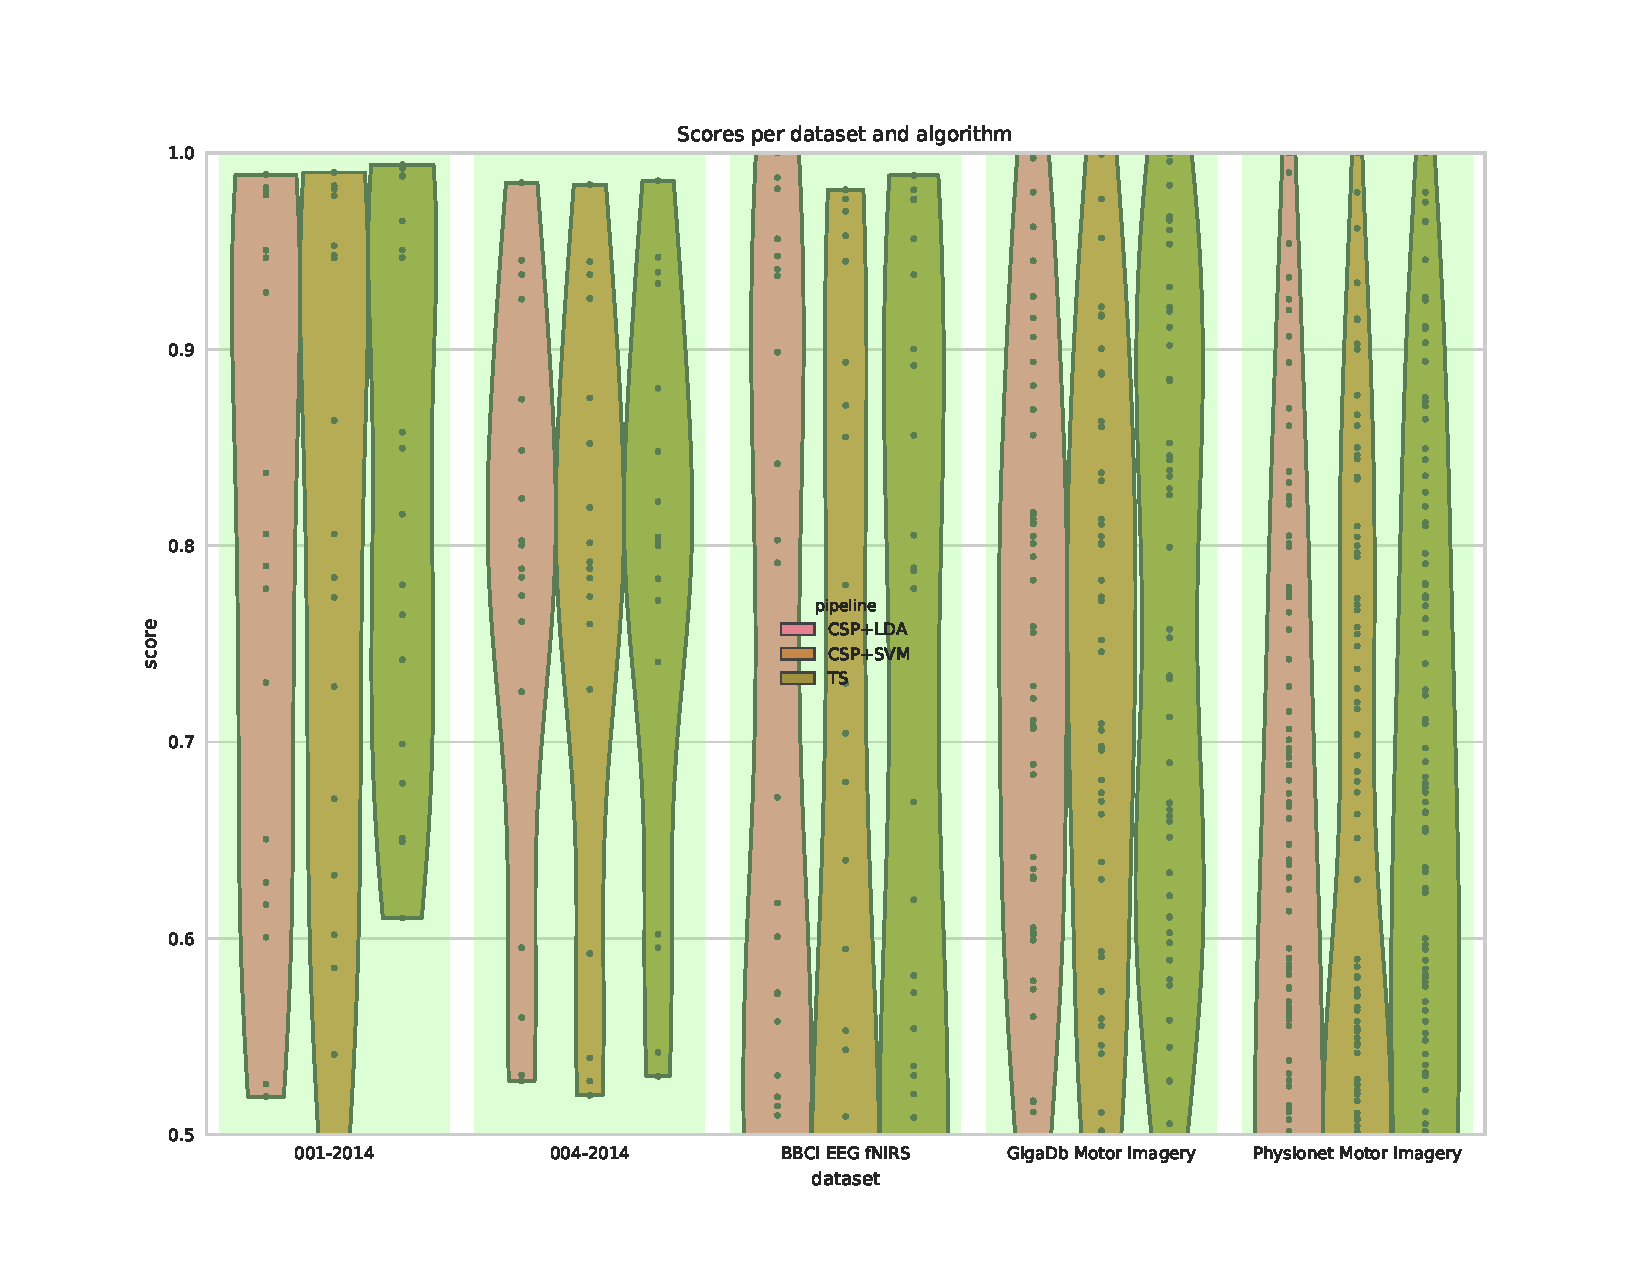
\includegraphics[width=\textwidth]{analysis/scores.pdf}
    \end{subfigure}%
     
    \begin{subfigure}[h]{0.45\textwidth}
        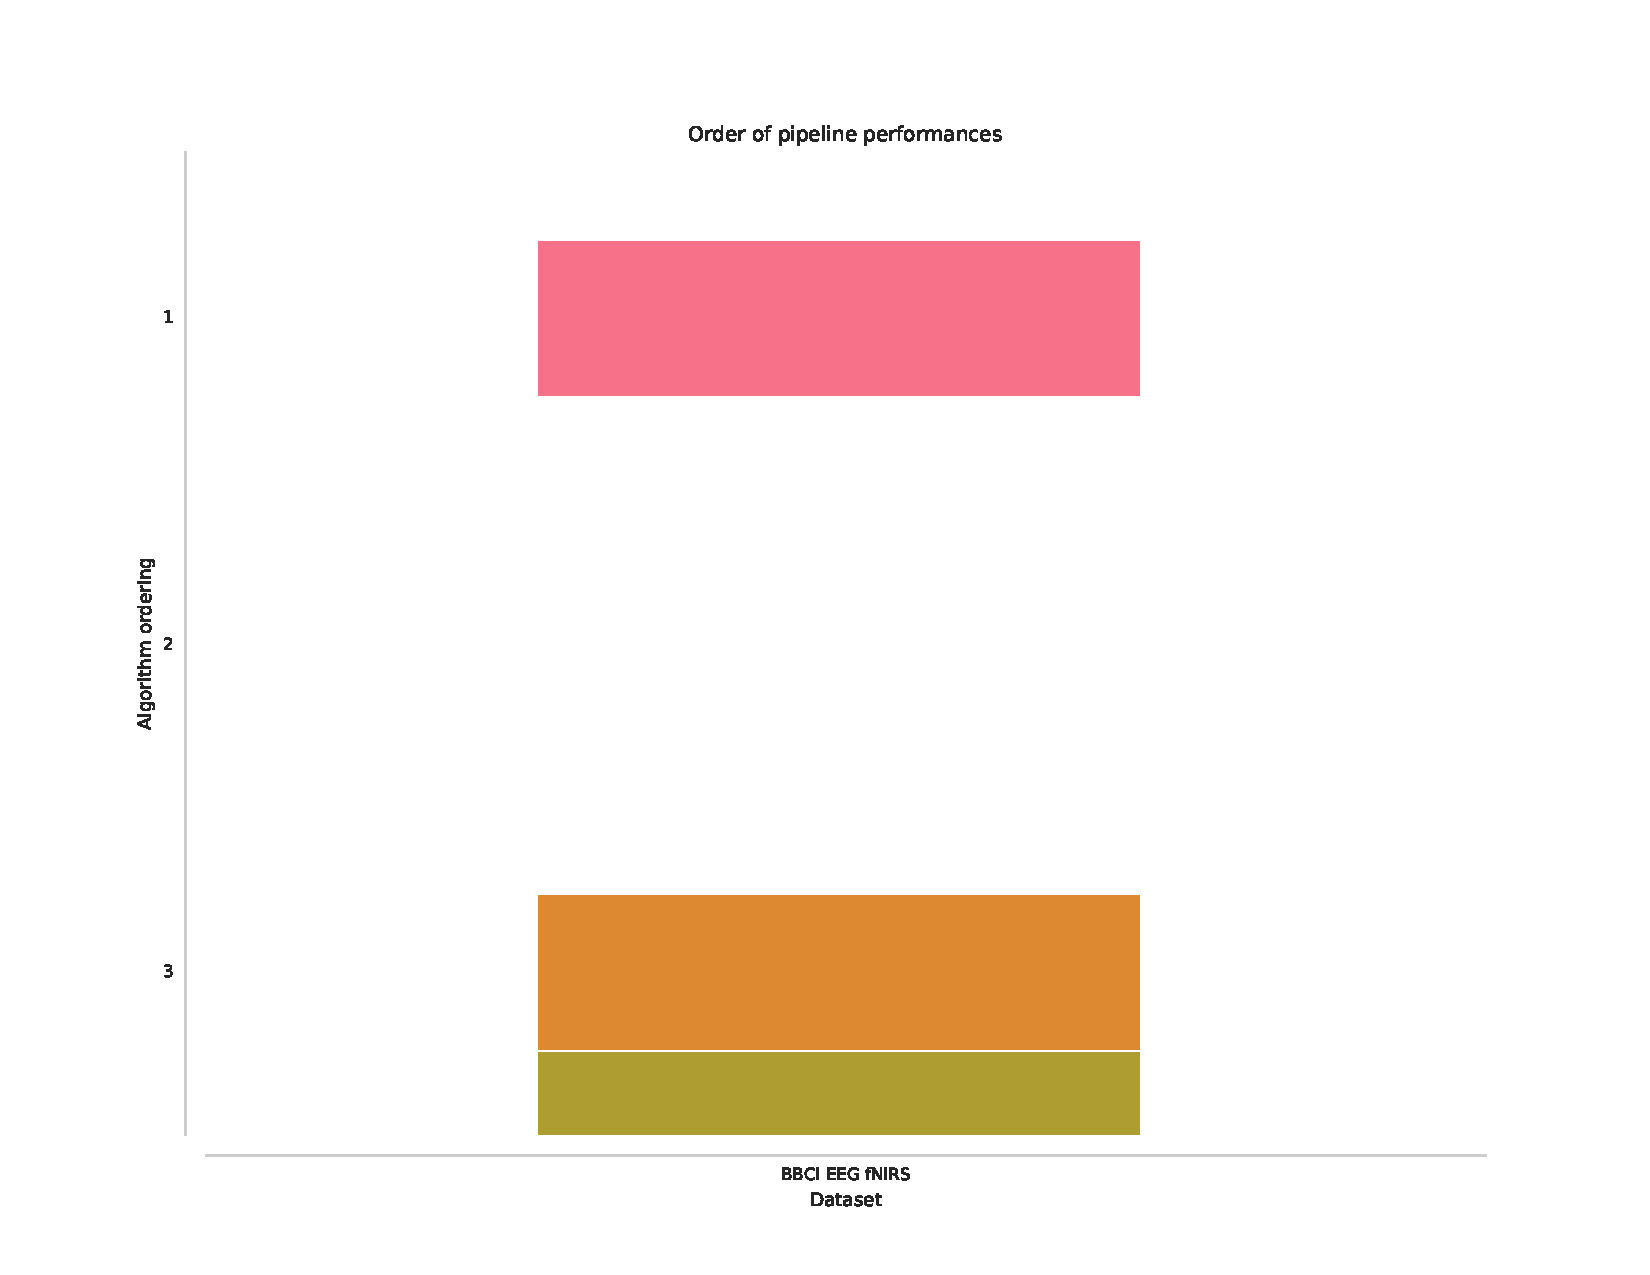
\includegraphics[width=\textwidth]{./analysis/ordering.pdf}
    \end{subfigure}
    \begin{subfigure}[h]{0.45\textwidth}
        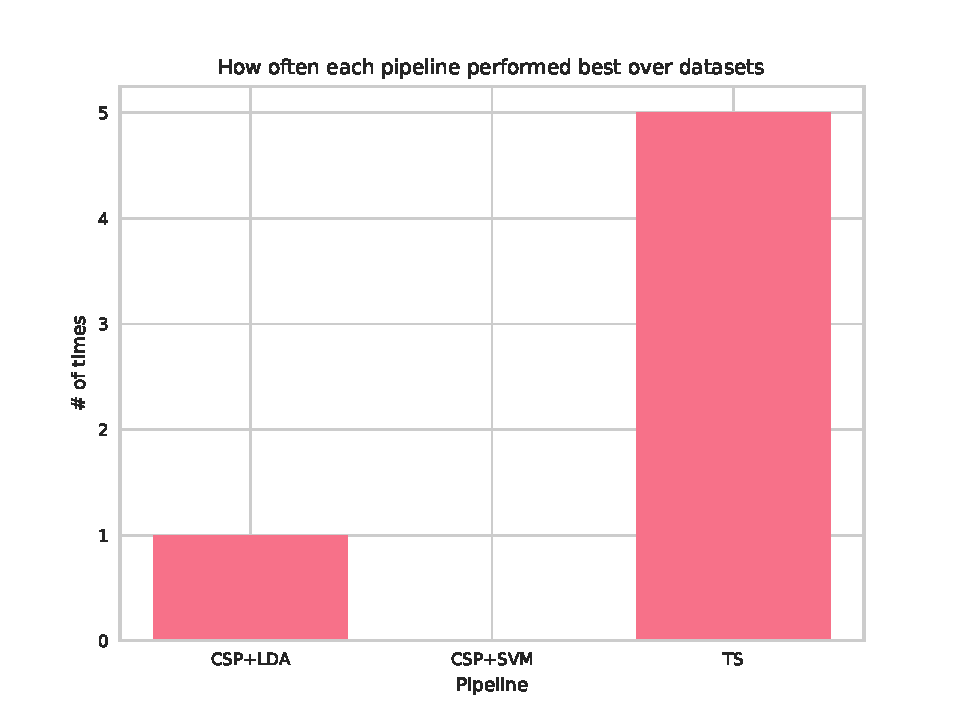
\includegraphics[width=\textwidth]{./analysis/summary.pdf}
    \end{subfigure}
    \caption{Caption place holder}
\end{figure*}
%%% Local Variables:
%%% mode: latex
%%% TeX-master: "main"
%%% End:
